\subsection{Hypothesis testing} \label{sec-hyp-test}


We now turn ourselves to applying the approximations developed in Section \ref{sec-pstar} on the problem of testing two nested Gaussian graphical models. More precisely, let $\G = (\Gamma, E)$ and $\G_0 = (\Gamma, E_0)$ with $E_0 \subset E$, we are interested in developing a test for the problem
\begin{equation} \label{eq-null-general-graph}
    H_0 : \Omega \in \S_{\succ 0}(\G_0)\ \ \t{ vs. }\ \ H_1 : \Omega \in \S_{\succ 0}(\G) \setminus \S_{\succ 0}(\G_0).
\end{equation}
The classical approach for testing this problem is to use the \textit{likelihood ratio test} based on the \textit{likelihood ratio statistic}. Given an observed covariance matrix $S_n$ constructed from a sample of size $n$, the likelihood ratio statistic is given by
\begin{equation*}
    \Lambda(S_n) = -2 \left[\ell(\hat\Omega_{\G_0}(S_n)) - \ell(\hat\Omega_\G(S_n))\right],
\end{equation*}
where $\hat\Omega_{\G_0}$ and $\hat\Omega_\G$ are the functions mapping an observed covariance matrix to the maximum likelihood estimators of the precision matrix under the model $\G_0$ and $\G$. Under regularity conditions and assuming that the $H_0$ is true, the distribution of $\Lambda(S_n)$ converges to a $\chi^2_d$ distribution with $d = |E| - |E_0|$. A hypothesis test in final sample can then be constructed by using the $\chi^2_d$ approximation to the distribution of $\Lambda(S_n)$.

In Eriksen \cite{eriksen1996tests}, the author gives a simple example for which we can demonstrate how this approximation fails when the sample size $n$ is not large enough. Consider two graphs $\G$ and $\G_0$ with $p = 4$ nodes such that $\G_0$ is a cycle and $\G$ is a chordal cover of $\G$. We are then interested in the following hypothesis test in Figure \ref{fig-test-cycle-vs-diamond}. Eriksen proposes an alternative test statistic for testing this class of problem which, in this examples is
\begin{equation} \label{eq-q-stat}
    Q(S_n) = \expf{-\Lambda(S_n) / n},
\end{equation}
which asymptotically follows a beta distribution $B((n - 3)/2, 1/2)$.



As we have seen in the previous section, the maximum likelihood estimator exists under both $H_0$ and $H_1$ almost surely if $n \geq 3$. We can then empirically evaluate the $\chi_2^d$ approximation to the distribution of $\Lambda(S_n)$ and $B((n - 3)/2, 1/2)$ approximation to the distribution of $Q(S_n)$ by sampling the statistics under the null hypothesis of a chordless cycle. For a given sample size $n \in \N$, we sample $N = 10000$ values $\lambda_1, \ldots, \lambda_N$ of the statistic $\Lambda(S_n)$ under the null hypothesis. With this sample, we can construct the empirical cumulative distribution function $\hat F_\Lambda$ which approximates the true cumulative distribution function of $\Lambda(S_n)$, as well as the sorted empirical probabilities $\hat p_{i} = \hat F_\Lambda(\lambda_{(i)})$. The empirical probabilities $\hat p_{i}$ can then be compared to the probabilities $\tilde p_i = F(\lambda_{(i)})$ where $F$ corresponds to the cumulative distribution function of either the $\chi^2_1$ approximation of $\Lambda(S_n)$ or the $B((n - 3)/2, 1/2)$ approximation of $Q(S_n) = \expf{-\Lambda(S_n) / n}$. Figure \ref{fig-diamond-vs-square-small}, displays this comparison. As we can see in the upper pane of Figure \ref{fig-diamond-vs-square-small}, the $\chi^2_1$ approximation is a poor approximation to the distribution of $\Lambda(S_n)$ while the $B((n - 3)/2, 1/2)$ approximation to the distribution of $Q(S_n)$ is accurate even for small sample sizes. Since we are interested in constructing a hypothesis test based on these approximation, the small probability region is of particular interest. In the lower pane of Figure \ref{fig-diamond-vs-square-small}, we see that the $\chi^2_1$ approximation is particularly bad for $n=5$ where a test at level $\alpha=0.05$ based on the $\chi^2_1$ approximation would have a true size of $0.1$.
\begin{figure}[tbp!]
    \begin{minipage}[c]{.45\linewidth}
        \centering
        $\ \ \ \ \ \ \ \ \ \ \ \ \ H_0$
        \newline
        \newline
        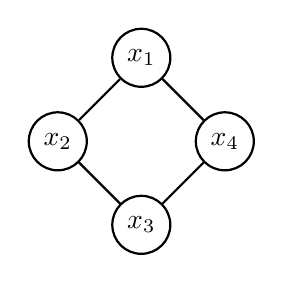
\begin{tikzpicture}[node distance={15mm}, thick, main/.style = {draw, circle}] 
            \node[main] (1) {$x_1$}; 
            \node[main] (2) [below left of=1] {$x_2$};
            \node[main] (3) [below right of=2] {$x_3$}; 
            \node[main] (4) [above right of=3] {$x_4$};
            \draw (1) -- (2);
            \draw (2) -- (3);
            \draw (4) -- (3);
            \draw (1) -- (4);
        \end{tikzpicture}
    \end{minipage}
    \begin{minipage}[c]{.1\linewidth}
        \centering
        $ $
        \newline\newline
        vs.
    \end{minipage}
    \begin{minipage}[c]{.45\linewidth}
        \centering
        $\ \ \ \ \ \ \ \ \ \ \ \ \ H_1$
        \newline
        \newline
        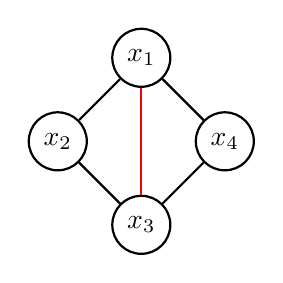
\begin{tikzpicture}[node distance={15mm}, thick, main/.style = {draw, circle}] 
            \node[main] (1) {$x_1$}; 
            \node[main] (2) [below left of=1] {$x_2$};
            \node[main] (3) [below right of=2] {$x_3$}; 
            \node[main] (4) [above right of=3] {$x_4$};
            \draw (1) -- (2);
            \draw (2) -- (3);
            \draw (4) -- (3);
            \draw (1) -- (4);
            \draw (1) edge[red] (3);
        \end{tikzpicture}
    \end{minipage}
    \caption{Simple hypothesis test proposed by Eriksen \cite{eriksen1996tests} for which the $\chi^2_1$ approximation to the likelihood ratio statistic fails.}
    \label{fig-test-cycle-vs-diamond}
\end{figure}
\begin{figure}[!tbp]
    \centering
    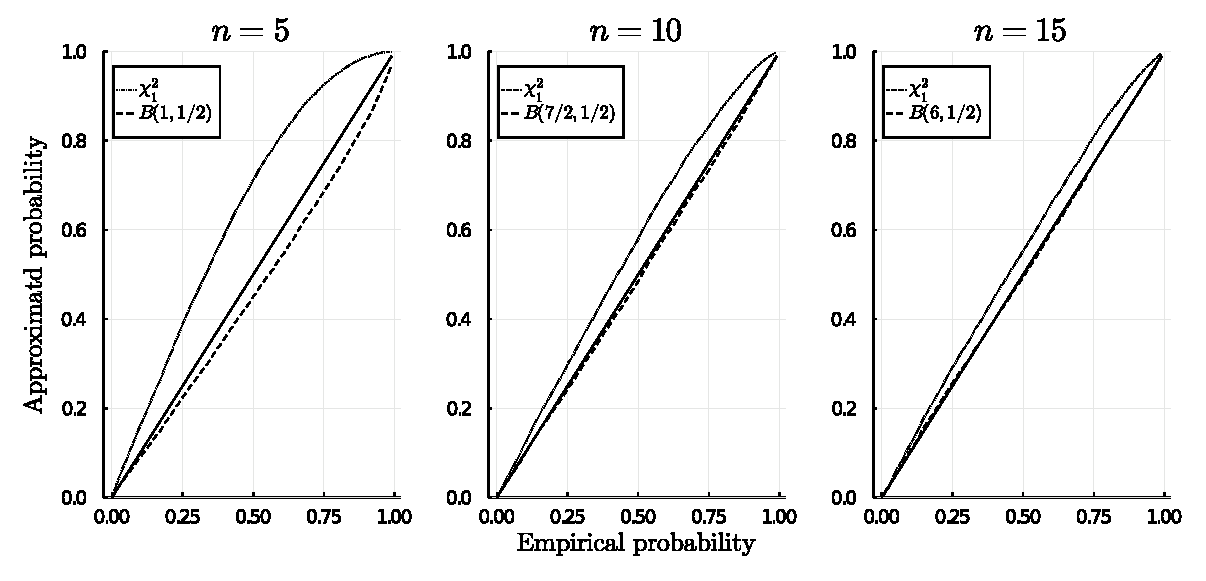
\includegraphics[width=16cm]{diamond_vs_square_0_1}
    \newline
    \newline
    \newline
    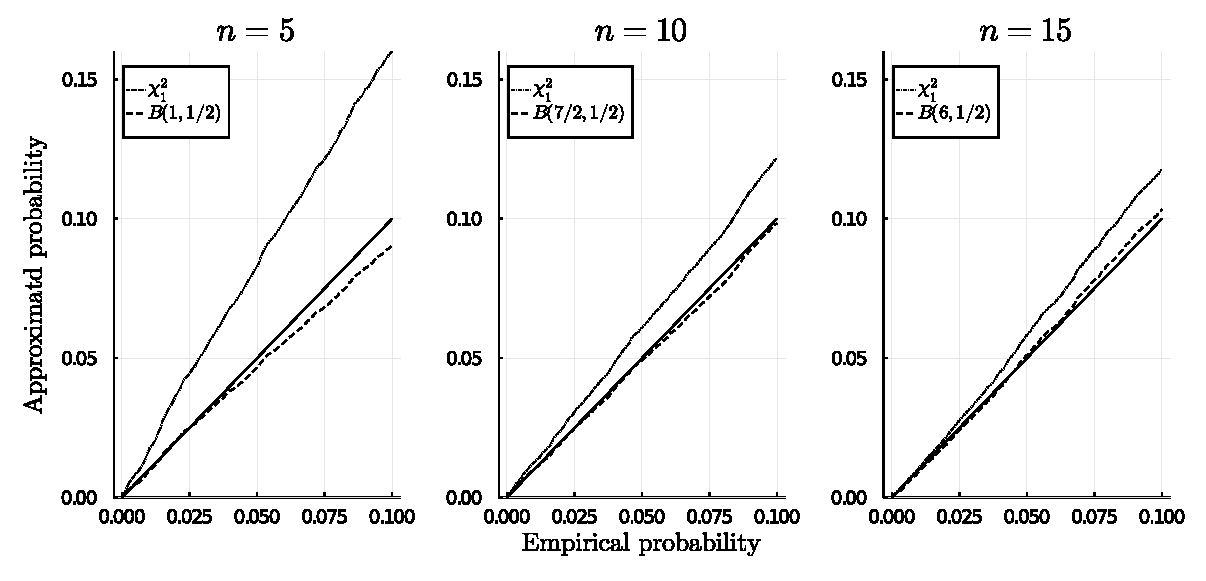
\includegraphics[width=16cm]{diamond_vs_square_0_01}
    \caption{Comparison of the $\chi^2_1$ approximation of the $\Lambda(S_n)$ statistic and Beta approximation of the $Q(S_n)$ statitistic from Eriksen \cite{eriksen1996tests} for testing the null hypothesis of a chordless cycle given a sample of $n = 5, 10, 15$ observations. As seen in the upper pane, the $\chi^2_1$ approximation poorly estimates the distribution of the $\Lambda(S_n)$ statistic for small and moderate sample sizes, while the $B((n - 3)/2, 1/2)$ approximation to the distribution of $Q(S_n)$ is accurate even for small sample sizes. This is particularly strong when focusing on small probability regions as we show in the lower pane where the difference of probability can be of approximately 50\%.}
    \label{fig-diamond-vs-square-small}
\end{figure}


While the $B((n - 3)/2, 1/2)$ approximation seems accurate, it is not yet clear where it comes from and why it works. In the rest of this section based on Eriksen \cite{eriksen1996tests}, we present the construction of this statistic as well as proof of convergence. In the following lemma from \cite[Theorem 3.1]{eriksen1996tests}, we apply the $p^*$ approximation to construct an accurate estimation to the density of the sufficient statistic $S$.

\begin{lemma} \label{lem-pstar-covariance}
    Let $\G$ be a graph, $\Omega \in \S_{\succ 0}(\G)$ and $S$ be a sample covariance matrix computes from a sample of size $n$ of the Gaussian graphical model associated to $\G$ with precision matrix $\Omega$. Then, the density $p(S; \Omega)$ of $S$ satisfies
    \begin{equation*}
        p(S; \Omega) = c \frac{|\Omega|^{n/2}}{|\hat\Omega_\G(S)|^{n/2}} |j_\G(\hat\Omega_\G(S)) |^{-1/2} \expfc{-\frac{n}{2} \trB{\Omega S}} (1 + O(n^{-3/2})),
    \end{equation*}
    where $c$ is a normalization constant, $\hat\Omega_\G(S)$ is the maximum likelihood of $\Omega$ assuming the graph $\G$ and given the data $S$, and $j_G$ is the observed information matrix given by
    \begin{equation} \label{eq-obs-info}
        j_\G(\Omega)_{a b} = \trB{\Omega^{-1} H_a \Omega^{-1} H_b} \t{ for all } a, b  \in E.
    \end{equation}
\end{lemma}

\begin{proof}
    Since $XX^\top$ is sufficient in the Gaussian graphical model, $S$ corresponds to the sample average of the sufficient statistic. Applying the $p^*$ approximation to $S$ as done in Section \ref{sec-pstar}, we have that the density of $S$ satisfies
    \begin{equation*}
        p(S; \Omega) = c |j_\G(\hat\Omega_\G(S))|^{-1/2} \expfc{\ell(\Omega; S) - \ell(\hat\Omega_\G(S); S)} (1 + O(n^{-3/2})).
    \end{equation*}
    Replacing the log-likelihood of the Gaussian graphical model in the above equation, we get
    \begin{align*}
        p(S; \Omega) 
        &\propto |j_\G(\hat\Omega_\G(S))|^{-1/2} \expfc{\ell(\Omega; S) - \ell(\hat\Omega_\G(S); S)} (1 + O(n^{-3/2})) \\
        &\propto |j_\G(\hat\Omega_\G(S))|^{-1/2} 
        \frac{|\Omega|^{n/2}}{|\hat\Omega_\G(S)|^{n/2}}
        \expfc{-\frac{n}{2}\left(\trB{\Omega S} - \trB{\hat\Omega_\G(S) S}\right)} (1 + O(n^{-3/2}))\\
        &\propto |j_\G(\hat\Omega_\G(S))|^{-1/2} 
        \frac{|\Omega|^{n/2}}{|\hat\Omega_\G(S)|^{n/2}}
        \expfc{-\frac{n}{2}\trB{\Omega S}} (1 + O(n^{-3/2}))
    \end{align*}
    where we use that $\hat\Omega_\G(S) S = 1_p$ and hence $\trB{\hat\Omega_\G(S) S} = p$ is constant. The formula for the observed infomation matrix can be easily verified by taking the appropriate derivatives of the log-likelihood.
\end{proof}

Before applying the result of Lemma \ref{lem-pstar-covariance} to the general problem of subgraph testing, we start with studying a special case. Consider a Gaussian graphical model with graph $\G = ([p], E)$ and the sub-model constructed by remove an edge $a \in E$ from $\G$. The sub-model is then the Gaussian graphical model associated to the graph $\G_0 = ([p], E_0)$ where $E_0 = E \setminus \eset{e_0}$. Without loss of generality, we assume $e_0 = \eset{1,2}$. The test statistic given in (\ref{eq-q-stat}) is then
\begin{align*}
    Q(S_n) 
    &= \expf{-\Lambda(S_n) / n}  \\
    &= \expf{2 \left[\ell(\hat\Omega_{\G_0}(S_n)) - \ell(\hat\Omega_\G(S_n))\right] / n} \\
    &= \expf{
        (\log |\hat\Omega_{\G_0}(S_n)| - \tr[S_n\hat\Omega_{\G_0}(S_n)])
        -    
        (\log |\hat\Omega_\G(S_n)| - \tr[S_n\hat\Omega_\G(S_n)])} \\
    &= \frac{|\hat\Omega_{\G_0}(S_n)|}{|\hat\Omega_{\G}(S_n)|},
\end{align*}
where we have used that $\tr[S_n\hat\Omega_{\G_0}(S_n)] = p$ is constant given any assumed graph. In the following theorem from \cite[Theorem 3.2]{eriksen1996tests}, we show that the $Q(S_n)$ statistic asymptotically follows a beta distribution with known parameters.

\begin{theorem} \label{thm-one-edge-less}
    Let $\G = ([p], E)$ be a graph with subgraph $\G_0 = ([p], E_0)$ with $E \setminus E_0 = \eset{e_0}$. Let $S$ be a sample covariance matrix computed from a sample of size $n$ of the Gaussian graphical model associated to $\G_0$ with precision matrix $\Omega_0 \in \S_{\succ 0}(\G_0)$. Then, the distribution of $Q(S_n)$ conditioned on observing $S_n$ is asymptotically
    \begin{equation}
        Q(S_n) \sim B\left(\frac{n - f(e_0) - 1}{2}, \frac{1}{2} \right)\ \ \ \ \t{ as } n \rightarrow \infty,
    \end{equation}
    where $f(\eset{i, j}) = |\t{bd}(i) \cap \t{bd}(j)|$.
\end{theorem}
\begin{proof}
    We can then construct approximations to the densities $p(S^{\G_0}; \Omega_0)$ and $p(S^{\G}; \Omega_0)$ by applying Lemma \ref{lem-pstar-covariance} in the Gaussian graphical models associated to $\G$ and $\G_0$ to get
    \begin{equation*}
        p(S^{\G_0}; \Omega_0) = c \frac{|\Omega_0|^{n/2}}{|\hat\Omega_{\G_0}(S^{\G_0})|^{n/2}} |j_{\G_0}(\hat\Omega_{\G_0}(S^{\G_0})) |^{-1/2} \expfc{-\frac{n}{2} \trB{\Omega_0 S^{\G_0}}} (1 + O(n^{-3/2}))
    \end{equation*}
    and
    \begin{equation*}
        p(S^\G; \Omega_0) = c \frac{|\Omega_0|^{n/2}}{|\hat\Omega_\G(S^\G)|^{n/2}} |j_\G(\hat\Omega_\G(S^\G)) |^{-1/2} \expfc{-\frac{n}{2} \trB{\Omega_0 S^\G}} (1 + O(n^{-3/2})).
    \end{equation*}
    Combining these results together allows us to approximate the density of $S_e$ conditioned on $S^{\G_0}$
    \begin{align*}
        p(S_{e_0}| S^{\G_0}; \Omega_0)
        &= \frac{p(S_{e_0}, S^{\G_0}; \Omega_0)}{p(S^{\G_0}; \Omega_0)} = \frac{p(S^{\G}; \Omega_0)}{p(S^{\G_0}; \Omega_0)}\\
        & \doteq \tilde c 
        \frac
            {|\Omega_0|^{n/2}|\hat\Omega_{\G_0}(S^{\G_0})|^{-n/2} |j_{\G_0}(\hat\Omega_{\G_0}(S^{\G_0})) |^{-1/2} \expfc{-\frac{n}{2} \trB{\Omega_0 S^{\G_0}}}}
            {|\Omega_0|^{n/2}|\hat\Omega_\G(S^\G)|^{-n/2} |j_\G(\hat\Omega_\G(S^\G)) |^{-1/2} \expfc{-\frac{n}{2} \trB{\Omega_0 S^\G}}}\\
        &= \tilde c 
        \frac
            {|\hat\Omega_\G(S^\G)|^{n/2} |j_\G(\hat\Omega_\G(S^\G)) |^{1/2}}    
            {|\hat\Omega_{\G_0}(S^{\G_0})|^{n/2} |j_{\G_0}(\hat\Omega_{\G_0}(S^{\G_0})) |^{1/2}}\\
        &= q^{n/2} \frac{|j_\G(\hat\Omega_\G(S^\G)) |^{1/2}}    {|j_{\G_0}(\hat\Omega_{\G_0}(S^{\G_0})) |^{1/2}}.
    \end{align*}
    where we used in the last step that $\Omega_0 S^\G = \Omega_0 S^{\G_0}$ which leads to the exponential terms canceling out. Since $w \xrightarrow{d} \chi^2_1$ is asymptotically ancillary, and $q = \expfc{-\frac{1}{2} w}$, $q$ is also asymptotically ancillary. Since $S^{\G_0}$ is a complete sufficient statistic assuming $\G_0$, $S^{\G_0}$ and $q$ are asymptotically independent by Basu's Theorem \cite{10.2307/25048259}. This means that asymptotically $p(S_{e_0}; \Omega_0) = p(S_{e_0} | S^{\G_0}; \Omega_0)$ for any $S^{\G_0}$ and we can chose $S^{\G_0}$ freely in the previous equation. Taking $S^{\G_0} = 1_p$ gives
    \begin{equation*}
        S^\G = 1_p + S_{e_0} H_{e_0} = \begin{pmatrix}
            1   & S_{e_0} & \\
            S_{e_0} & 1 & \\
                &   & 1_{p-2}
        \end{pmatrix}.
    \end{equation*}
    Since $S^{\G_0}$ and $S^\G$ are positive definite, they are their own positive definite completion and we have $|\hat\Omega_\G(S^\G)| = |S^\G|^{-1} = (1 - S_{e_0}^2)^{-1}$ and $|\hat\Omega_{\G_0}(S^{\G_0})| = |S^{\G_0}|^{-1} = 1$, giving $q = 1 - S_{e_0}^2$. A change of variable from $S_e$ to $q$ has Jacobian $(1 - q)^{-1/2}$ and the density of $q$ can be given by
    \begin{equation} \label{eq-proof-almost-done}
        p(q) \doteq \hat c q^{n/2} |j_{\G}(\hat\Omega_{\G}(S^{\G})) |^{-1/2} (1 - q)^{-1/2},
    \end{equation}
    for some normalizing constant $\hat c$.

    We now bring our attention to computing the determinant of the observed information matrix given in (\ref{eq-obs-info}) with $\Omega^{-1} = 1_p + S_e H_e$. Let $a, b \in E$, we start by noting that for any $S \in \S(\G)$ and $i, j \in [p]$
    \begin{equation*}
        (SH_a)_{ij} = \begin{cases}
            & S_{i \bar j}\ \ \t{ if } j \in a\\
            &0\ \ \ \ \  \t{otherwise}
        \end{cases}
        \ \ \ \t{ and }\ \ \ \ \ 
        (SH_b)_{ji} = \begin{cases}
            & S_{j \bar i}\ \ \t{ if } i \in b\\
            &0\ \ \ \ \  \t{otherwise}
        \end{cases},
    \end{equation*}
    where $\bar j \in a$ and $\bar i \in b$ are such that $\eset{j} \cup \eset{\bar j} = a$ and $\eset{i} \cup \eset{\bar i} = b$. Using this in the expression of $j_\G(S)_{ab}$, we get
    \begin{equation} \label{eq-tr-sum}
        \trB{SH_aSH_b} = \sum_{i=1, j=1}^p (SH_a)_{ij}(SH_b)_{ji} = \sum_{(i, j) \in a \times b} S_{i \bar j} S_{j \bar i} = \sum_{e \in a \times b} S_e S_{\bar e},
    \end{equation}
    where the last equality only involves re-indexing and re-ordering the sum. We now inspect the different $a, b$ for which the summand $S_eS_{\bar e}$ is non-zero. Setting $s = S_{e_0}$, we have $S = 1_p + s H_{e_0}$ and hence for any $e \in E$
    \begin{equation*}
        S_e = \begin{cases}
            &1\ \ \t{ if } e = \eset{ i } \t{ for } i \in [p]\\
            &s\ \ \t{ if } e = e_0\\
            &0\ \ \t{ otherwise}.
        \end{cases}
    \end{equation*}
    Thus, the summands $S_e S_{\bar e}$ of (\ref{eq-tr-sum}) are non-zero if and only if both $e$ and $\bar e$ are either $\eset{i}$ for some $i \in [p]$ or equal to $e_0$. Without loss of generality, we will assume that $e_0 = \eset{1, 2}$. This leaves us with the following cases. 

    Case 1. $e = \bar e = \eset{1, 2}$. This can only happen if $a = \eset{1}$ and $b = \eset{2}$, in which case
    \begin{equation*}
        j_\G(S)_{\eset{1} \eset{2}} = \sum_{e \in \eset{1} \times \eset{2}} S_e S_{\bar e} = S_{\eset{1, 2}}S_{\eset{1, 2}} = s^2.
    \end{equation*}

    Case 2. $e = \eset{1, 2}$ and $\bar e = \eset{i, j}$ with $i \neq j$ (or the opposite). Then we must have $a = \eset{1, i}$ and $b = \eset{2, j}$ and
    \begin{equation*}
        j_\G(S)_{\eset{1, i} \eset{2, j}} = S_{1 2}S_{i j} + S_{1 j} S_{i 2} + S_{i 2} S_{1 j} + S_{i j} S_{1 2} = 0,
    \end{equation*}
    since we assumed that $S = 1_p + s H_{e_0}$.

    Case 3. $e = \eset{1, 2}$ and $\bar e = \eset{i}$ (or the opposite). This is the case when $a = \eset{1, i}$ and $b = \eset{2, i}$ and we get
    \begin{equation*}
        j_\G(S)_{\eset{1, i} \eset{2, i}} = 
        S_{1 2}S_{i i} + S_{1 i} S_{i 2} + S_{i 2} S_{1 i} + S_{i i} S_{1 2} = 2 s,
    \end{equation*}
    since $S_{i i} = 1$, $S_{1, 2} = s$ and $S_{i 1} = S_{i 2} = 0$. Note that since the matrix $j_\G$ is indexed by edges in $\G$, the cases $a = \eset{1, i}$ and $b = \eset{2, i}$ are only relevant if $a, b \in E$ and so this case only for $i \in C = \t{bd}(1) \cap \t{bd}(2)$.

    Case 4. $e = \eset{i}$ and $\bar e = \eset{j}$. This only happens is $a = b = \eset{i, j}$, which, again using that $a, b \in E$ and $S = 1_p + sH_{e_0}$ gives
    \begin{equation*}
        j_\G(S)_{\eset{i, j} \eset{i, j}} = \begin{cases}
            &S_\eset{i, i}S_\eset{i, i} = 1\ \ \ \ \ \ \ \ \ \ \ \ \ \ \ \ \ \ \ \ \ \ \ \ \ \ \ \  \t{ if } i = j\\
            &2S_\eset{1 1}S_\eset{2 2} + 2S_\eset{1 2}S_\eset{1 2} = 2 + 2s^2\  \t{ if } \eset{i, j} = \eset{1, 2}\\
            &2S_\eset{i,i} + 2S_\eset{i, j} = 2\ \ \ \ \ \ \ \ \ \ \ \ \ \ \ \ \ \ \ \ \  \t{ otherwise.}
        \end{cases}
    \end{equation*}
    This shows that $j_\G(S)$ is a block diagonal matrix with blocks each equal to one of the following matrices
    \begin{equation*}
        A = \bordermatrix{~ & \eset{1} & \eset{2} & \eset{1, 2} \cr
            \eset{1} & 1 & s^2 & 2s \cr
            \eset{2} & s^2 & 1 & 2s \cr
            \eset{1, 2} & 2s & 2s & 2 + 2s^2 \cr
        }
        \ \ \ \ \ \ \ \ \ 
        B_i = \bordermatrix{~ & \eset{1, i} & \eset{2, i} \cr
            \eset{1, i} & 2 & 2s \cr
            \eset{2, i} & 2s & 2 \cr
        }, i \in C.
    \end{equation*}
    Since $|A| = 2 (1-s^2)^3$ and $|B_i| = 4(1-s^2)$ for $i \in C$, we have that the determinant of the observed information $\abs{j_\G(1_p + sH_{e_0})} \propto (1-s^2)^{3 + |C|} = (1 - S_{e_0}^2)^{3 + f(e_0)} = q^{3 + f(e_0)}$. Replacing this in (\ref{eq-proof-almost-done}) gives
    \begin{align*}
        p(q) 
        &\doteq \hat c q^{n/2} |j_{\G}(\hat\Omega_{\G}(S^{\G})) |^{-1/2} (1 - q)^{-1/2}\\
        &\propto q^{n/2} q^{-(3 + f(e_0))/2} (1 - q)^{-1/2} \\
        &= q^{(n - f(e_0) - 3)/2}(1-q)^{-1/2}.
    \end{align*}
    Since the density of a $B(\alpha, \beta)$ distribution is proportional to $q^{\alpha-1}(1-q)^{\beta-1}$ we have that $q$ asymptotically follows a $B((n - f(e_0) - 1)/2, 1/2)$ distribution.
\end{proof}

This construction can be generalized to the case where $d = |E \setminus E_0| > 1$. Let $E_- = E \setminus E_0 = \eset{e_0, \ldots, e_{d-1}}$, we define for $i = 1, \ldots, d-1$ the subgraphs $\G_i = ([p], E_i)$ with $E_i = E_{i-1} \cup \eset{e_i}$. Then, the $Q(S_n)$ statitistic can be decomposed as 
\begin{align*}
    Q(S_n) 
    &= \frac{|\hat\Omega_{\G_0}(S_n)|}{|\hat\Omega_{\G}(S_n)|}
    = \frac{|\hat\Omega_{\G_0}(S_n)|}{|\hat\Omega_{\G_{d-1}}(S_n)|} \\
    &= \frac{|\hat\Omega_{\G_0}(S_n)|}{|\hat\Omega_{\G_1}(S_n)|}
    \frac{|\hat\Omega_{\G_1}(S_n)|}{|\hat\Omega_{\G_2}(S_n)|}
    \ldots
    \frac{|\hat\Omega_{\G_{d-2}}(S_n)|}{|\hat\Omega_{\G_{d-1}}(S_n)|}
    =: Q_{0,1}(S_n)Q_{1,2}(S_n) \ldots Q_{d-2, d-1}(S_n),
\end{align*}
where $Q_{i, i+1}(S_n)$ corresponds to the test statistic for testing the submodel $\G_i$ in $\G_{i+1}$. Applying Theorem \ref{thm-one-edge-less} to each $Q_{i, i+1}(S_n)$ gives that, asymptotically
\begin{equation*}
    Q_{i, i+1}(S_n) \sim B\left(\frac{n - f(e_i) - 1}{2}, \frac{1}{2} \right) =: B(\alpha_i, 1/2)
\end{equation*}
where $f(e_i) = |\t{bd}(j) \cap \t{bd}(k)|$ for $e_i = \eset{j, k}$ is to be evaluated in the graph $\G_{i+1}$. Hence $Q(S_n)$ is asymptotically distributed as the product of independent $B(\alpha_i, 1/2)$ random variables.
